\documentclass{article}
\usepackage{cs6850}

\renewcommand\maketitle{
\begin{flushleft}
{%
\large{%
Benjamin Greenman,
Hersh Mehta
\hfill
CS6850: Reaction Paper
\\\texttt{\{blg59, hpm36\}} \hfill \today
}}\\
\hrulefill
\end{flushleft}
}

\begin{document}
\maketitle

\section{Introduction}
%% Introduce topic
%% - what is herding
Financial markets are commonly modeled by a set of independent actors who combine public and private information in order to make investments.
Public information is, as the name suggest, available to all decision-makers and private information is unique to each.
A minimum of information sharing is expected, perhaps inferred by analyzing an individual's past spending, but for the most part private information remains so.
At no point does all private information become public, creating an even playing field where rational agents will make identical decisions.
The market is always characterized by information asymmetries.

These models carry the assumption that individuals' choices are strongly guided by their private information.
However, this assumption has been contradicted by empirical findings. 
Numerous studies have found that investors do not always act as individuals, guided by private information, but rather exhibit a tendency for collective action.
Investors, in practice, often act as a herd.
Cont and Bouchad (1992) cite evidence of herding among fund managers and financial analysts in domestic markets \cite[174]{cont}.
Bikhchandani and Sharma (2000) present similar evidence from data in emerging Eastern markets \cite{bikhchandani}.
Herding, the phenomena where all or most actors in the market converge upon a single decision, occurs much more often than we might naively expect.

Reasons for herding are myriad, and will not be discussed in great depth here.
A great many psychological and economic factors might influence an individual trader's decision to herd. 
Rather than enumerate these we present only what is necessary to understand the models.
Additionally, we do not focus on the outcomes of herding.
The natural assumption is that herding is irrational, a poor strategy compared to using private information; however, there are a number of cases where herding is the optimal strategy.

Our primary concern is modeling herd behavior.
The motivation for herding and the consequent outcome are only important insofar as they dictate the constraints of accurate models.
We seek to identify whether certain decisions are the product of herding or not, and to predict when herding will guide other choices.
Sections 2 and 3 analyze the models presented in two prior studies on herding, noting where they have succeeded and where they have fallen short. 
Section 4 summarizes our ideas for future work and section 5 presents a small analytical example.

Our approach in choosing papers to read for this topic was to find one established, canonical paper that has had a significant influence on future works, and a newer paper offering modern insight and a more refined model.
From the former, we sought a summary of the phenomena and problem and an intuitive, uncluttered model upon which to test data.
We hoped this model would give a simple measure on one or two dimensions, to provide firm ground on which to build more intricate experiments.
Then from the latter paper, we wanted a more focused effort into solving a particular problem, to give an indication of which open questions remain pertinent today.
We expected the model in the newer paper to be more intricate, better tailored to answering a particular question or analyzing a particular structure of market as opposed to the more general, canonical model.

%% 2013-10-24: I think 'to this end' is much better, much less insulting than 'however', but let's figure out paper A before doing that shit.
To this end we have read Cont and Bouchad (2000), which presents a simple randomized model for herding, and Boorz et. al. (2013), which critiques the current state of research and applies herding techniques to high-frequency data.
%% To this end we have read Cont and Bouchaud (2000), which is a well-cited work which presents the first model of herding based on a randomized graph, and Lin et. al. (2009), which provides a good critique of existing models and offers a suggestion for a new model addressing the demands of high-frequency trading networks.
For additional background we reference Bikhchandani and Sharma (2001), an IMF paper which summarized the phenomena and provided empirical data on herding in emerging markets, and a few other related works.

%% Summarize sources
%% - what's the main technical content
%% - why's content interesting in relation to the corresponding section of the course
%% - what are some weaknesses of the papers, how can they be improved
%% - what are some promising future questions, how could they be answered (what're we gonna do for research)
\section{Review of Cont \& Bouchaud}
\subsection{Summary}
Cont and Bouchad (2000) did not set out to study herding per se, but rather to explain a curious observation.
Empirical data on the distributions of stock prices considerably differed from the expected Gaussian distribution: instead of a normal curve, the data showed heavy tails, indicating high kurtosis \cite{cont}.
These tails were known to have been caused by large fluctuations in prices, but the cause of the fluctuations was unknown.
Prior work by Cutler (1989) and Shiller (1989) had established that the arrival of information or variations in fundamental economic variables did not always lead to heavy-tailed distributions, which led the authors to hypothesize that herding might be a cause.
Thus they developed a new herding model with the hope that its underlying distribution would match those found in the data.

Before presenting their model, the authors summarize previous models and how those models guided the present design.
%% first set
One problem they wanted to avoid was the assumption that decisions take place sequentially.
A natural herding model, proposed by Bikhchandi (1992) has investors take turns making decisions based off the state of the market and competitors' past actions.
While easy to understand, this type of model is not realistic. 
Stock markets are not characterized by sequential actions; trades take place in a fast-paced information-asymmetric environment. 
There is no time to stop, as if in a board game, and analyze everything that has occurred thus far before choosing the next move. 
Trading is by nature asynchronous.
However, an earlier non-sequential model by Orl\`{e}an (1995) proved insufficient because it gave all players an equal likelihood of copying one another.
Hoping to avoid that pitfall, the authors' model uses a randomized communication structure to give players unfair access to private information.

Another issue is the intricacy of the model.
The authors critique earlier work by Bat (1997) for being too complex, for having so many parameters that determining causation was difficult and comparison against empirical data was overly tedious and had too many of failure \cite{cont}.
Hence their model is simple and uncluttered: a set of $N$ agents choose to buy, sell, or hold a single asset.
At the start of the simulation, agents are formed into groups by creating edges with probability $c/N$ for some connectivity parameter $c \in [0,1]$.
These clusters are the herds for the rest of the simulation, which is then executed, logging returns throughout.

After introducing their model, the authors show, via a formulaic argument, that it is characterized by the same heavy, non-Gaussian tails as the empirical data. 
At small timescales, their model yields heavy tails, just like the data, and these smooth out to become increasingly Gaussian as the timestep increases.
This clears the deficiencies present in older models. 
However, the authors do not test their model on any real or simulated data, leaving instead a clear avenue for future work.
That said, a powerful testament to this model's success is the extent to which it has been cited in subsequent papers.
Whether those authors agreed or disagreed with its methodology or accuracy, they at least found it suitable for discussion.
%% implications of herding for for market demand + price fluctuations

\subsection{Main Technical Content}
The formalization of a randomized herding model and its corresponding analysis constitute the main technical content of this paper.
The authors identified problems with past approaches and addressed these in their model, using the best of past work to guide the new approach.
Randomization was a novel approach taken in this work, and these ideas have been incorporated and emulated in future models \cite{lin}.
Furthermore, the analysis presented here is detailed and comprehensive despite the lack of data, offering convincing evidence that the model does indeed give heavy-tailed distributions much like those observed empirically.

\subsection{Relation to coursework}
This paper, indeed this topic, brings together a variety of topics from this course. 
Concepts dealt with explicitly in this paper are random graphs and game-theoretic models.
Indeed, what sets this model apart from its contemporaries is that it was randomized, which was ultimately a better technique for dealing with trading networks.
Information cascades are addressed here as well, though they are not the core focus.
The literature, at this point in time, assumes that information cascades cause herding.
Herding is a primarily psychological phenomena that carries through individuals in the market.
This model challenges that assumption slightly by rejecting sequential models of herding, but it is not for another decade that the legitimacy of the information cascade hypothesis is seriously questioned \cite{lin}.

\subsection{Weaknesses and open questions}
%% This model does not take into account
An obvious failure of this paper is its the lack of simulation or analysis.
The model is thoroughly defined and discussed at great length, but never actually tested. 
Since the ultimate goal of a herding model is how well it describes behaviors we observe in the data, the lack of emprirical testing, even on simulated data, is disappointing.

Another issue is that the herds in this model, once formed, never change. 
Certainly, this is not how herding occurs in practice. 
Inviduals are free to drop in and out of particular herds as time progresses; there is no mechanism binding them to one group alone.
A better randomized model might let individuals join or leave groups with some nonzero probability at discrete time intervals.
Determining suitable probabilities for the initial step to join a group, or for group cohesion among members who have already joined, may indeed be a rich project for a future study.

%% TODO pick out some failures with the model itself
The authors also note that while their model is a threshold model, thresholds are uniform across all participants. 
Randomizing the thresholds may lead to more realistic outcomes. 
Of course, this hypothesis would have to be tested against the current model on some dataset, preferably large and taken from real markets, which again begs the question of a more formal analysis.

\section{Review of Boortz et. al.}
\subsection{Summary}
  Boortz et. al. summarizes the recent efforts of a group of German researchers towards linking the empirical and theoretical perspectives of herding. 
  Research on herding, they claim, has been divided for too long into two separate empirical and theoretical realms.
  Theoreticians have developed models in line with the evolution of modern securities markets; as the pace and style of trading has changed, so have the models.
  However, these models are not applicable to the corresponding empirical context.
  They focus on individual investor level herding in a tick-by-tick trading context \cite[2]{boortz}.
  Data at this level of detail is difficult to obtain, largely due to privacy regulations but because individual motives and actions are difficult to record.
  Certainly, this was a problem we faced in writing this reaction piece. Data of poor quality was available for sale or signup, but high-quality, high-frequency data took a great deal of effort to acquire.
  Empirical studies on the other hand are data-driven, and therefore focus on aggregates over relatively large blocks of time.
  Depending on the data available, published results have developed from conclusions based on weekly or even yearly aggregates.\footnote{
    Here ``aggregates'' should be taken to mean the window over which data are compared. 
  }
  Granted, this may be appropriate for slow moving, established markets, but it is certainly not accurate for high-frequency or emerging markets.
  Markets in which millions of trades occur every second demand more granular measurements than by day or by week.
  Thus we have one issue: that theoretical and practical results are not synchronized.

  The authors seek to address this discontinuity by giving theoretical and empirical results within the same paper.
  First, they present a dynamic model for measuring the intensity of herding in a fast-paced market.
  Next, they run this model on simulated data and generate hypotheses from it.
  Finally, they test these hypothesis on up-to-date and relevant market data, recorded during the 2007 financial crisis and provided by the German Federal Financial Supervisory Authority \cite[3]{boortz}.
  The output here is used to validate the hypothesis, and then the authors present their conclusions.
  This approach differs from the methodology of other works, including that of Cont and Bouchaud, above, making for an interesting and influential study.

\subsection{Herding Measure}  
  Interestingly, the model used here is simple, operating on very few parameters. 
  Only one asset is traded between buyers and sellers, and investors are either bucketed into two groups: informed and noisy \cite[5]{boortz}.
  Noisy traders randomly buy a stock at each opportunity.
  Informed traders make decisions based on the past and current state of the market, have the choice of buying or holding at each opportunity, and are evaluated against a few criteria to determine whether they have exhibited herd behavior.
  The folowing criteria describe when a trader exhibits buying heard behavior (there are symmetric conditions for seller hearding).
  \begin{itemize}
  \item 
    The trader is informed
  \item
    The trader chooses to buy at the current time
  \item 
    The trader either sold or did not act at the previous time
  \item 
    The number of buyers currently in the market exceeds the number of sellers (informed or otherwise)
  \end{itemize}
  The usefulness and applicability of the model stems from its simplicity. 
  As noted in the authors' introduction, theoretical models had become advanced and multi-faceted, but in doing so had grown apart from contemporary empirical work.
  While developing their model, the authors were conscious of the need to apply the model to real data.
  Hence the resulting model is easily applicable to the current data, and will adapt to more results for future studies.

\subsection{Main Technical Content}  
  The definition and rigorous application of a herding measure for high-frequency data are the main contributions of this work.
  Although their model is but a slight modification of one developed by Park and Sabourian (2007), using only a less restrictive definition of when herding has occurred, it is still a useful contribution.
  What makes this model particularly useful for analyzing high frequency data is its dynamic nature.
  It measures the correlation between traders' purchasing behavior in discrete time steps, rather than all at once after synthesizing all the data.
  Additionally, this measure differentiates between traders who follow others and who follow themselves, taking advantages of the investor-specific information available to the authors \cite{boortz}. 
  
  This usefulness is affirmed in the model's application to the simulated and actual data.
  Indeed, the analysis is itself a significant technical contribution.
  This paper presents a model for how future ideas ought to be presented: first develop a model, then test it on simulated data, finally run it on live data.
  While seemingly common sense, few works in this subject have actually followed this scientific approach.

\subsection{Relation to coursework}
  %% Information cascades
  %% Randomized parameters
  Like Cont and Bouchaud, this paper discusses information cascades, simple game theoretic models, and randomized networks.
  While they do not incorporate all these dimensions directly into their model, the authors do mention them as opportunities for expansion.
  The parameters they do focus on are market stress and information risk, both of which are directly linked to the phenomena of information cascades \cite{boortz}.
  
  Increased market stress, according to the authors, is associated with greater buyer uncertainty and a generally pessimistic economic outlook.
  The authors make inferences about market stress by analyzing data before and during the economic crisis. 
  They assume market stress to be contagious, and to spread quickly through the market as news travels through public channels.
  
  Information risk denotes the likelihood one is trading with a party that has private information regarding the assert.
  This parameter models the expected returns of herding; if your competitors have access to priviledged information, you can expect to do better following their lead instead of guessing blindly.
  When it rises, the authors expect traders to herd together in order to minimize their risk. 


\subsection{Weaknesses and open questions}

Unlike previous works on herding, this paper dealt exclusively with high-frequency data. 
High-frequency trading systems are interesting in that they are not driven by humans, who are subject to emotions and stress, but rather by machines executing trading algorithms. 
This raises an interesting question, which the paper authors did not fully address.
Prior work treated herding as a psychological effect, made possible by human fear and a desire to combat uncertaintly. 
Herding was considered an irrational decision, an instinctual drive to ignore private data which nearly always led to inferior results. 
Bikhchandani and Sharma (2001) talked specifically about reputation-based and compensation-based motivations for herding. 
The former refers to how much trust traders have in their fund manager is; the latter describes the individual tendency to herd when their income is based on their ability to avoid failure \cite{bikhchandani}.
Both are specifically human phenomena.
Now we have trading machines, which feel none of the emotion or fear human traders did. 
Yet herding still exists\textemdash despite being immune to the hypothesized causes of herding, machines exhibit the same, supposedly poor judgement.
Hence there must be benefits to herding, at least, much more than early research gave it credit. 

More recent works have understood that herding becomes the rational choice in some cases. 
Boorz et. al. recognize that herding is a viable strategy to deal with information asymmetries or to minimize losses \cite{boortz}.
Lin et. al. found that herding increased in times of abundance, much like how stock bubbles form and grow \cite{lin}.
However, there is not yet a satisfactory explanation for when herding occurs in high-frequency markets.
If machines are making the trades, then there must be observable parameters that indicate when to lead and follow.
These measures are already encoded in the algorithm's logic. 
Yet the paper which brings together and generalizes these criteria apparently has yet to be written.

\section{Proposal}
%% Give a proposal for a model, or a new algorithm. Can extend / vary something from papers

High-frequency trading (HFT) is a relatively new phenomena, but has revolutionized financial markets.
The modern trading floor is much different from the one analyzed by Cont and Bouchad.
To this end, we need a new model of herding corresponding to the new model of transactions.
Boortz et. al. provided a solid foundation for analyzing HFT data, but their model is relatively simplistic. 
More detailed, more focused models should be experimented with.
Taking the same approach outlined by Boortz et. al., we seek to introduce a new model for analyzing herd behavior and apply it to high frequency data. 

In developing the our new model, we hope to modify the existing model, first proposed by Park and Sabourian (2011), by introducing a randomized parameter.
Some possible avenues for exploration include modifying the signals for informed traders, changing the algorithm for noise traders, pre-assigning groups in the same manner as Cont and Bouchaud, and adding ``herd'' traders who always follow the crowd regardless of their signal or other historical data.

\section{Analysis}
As a preliminary experiment, we ran a simulation inspired by Boortz et. al. but with a randomized signal structure.
We created the same premises as their simulation for testing the effects of information risk, namely, a pool of traders who are partitioned based on parameter $\mu$ into informed and noise traders, and a series of stocks which assume one of three possible values.
Using the same noise trader behavior and herding condition, we simulated trading for each stock over 100 time steps.
The difference we introduced was that traders, rather than working with one private signal determined at the start of the simulation, received a new, randomized signal before making each trade.
This modification represents a primitive means of accounting for dynamic private information and trading algorithms. 
Later, we will refine this perturbation; for now, we simply experiment to see how the outcomes are affected if traders are given slightly more autonomy.

\begin{figure}
  \begin{minipage}{0.5\textwidth}
    \begin{flushleft}
      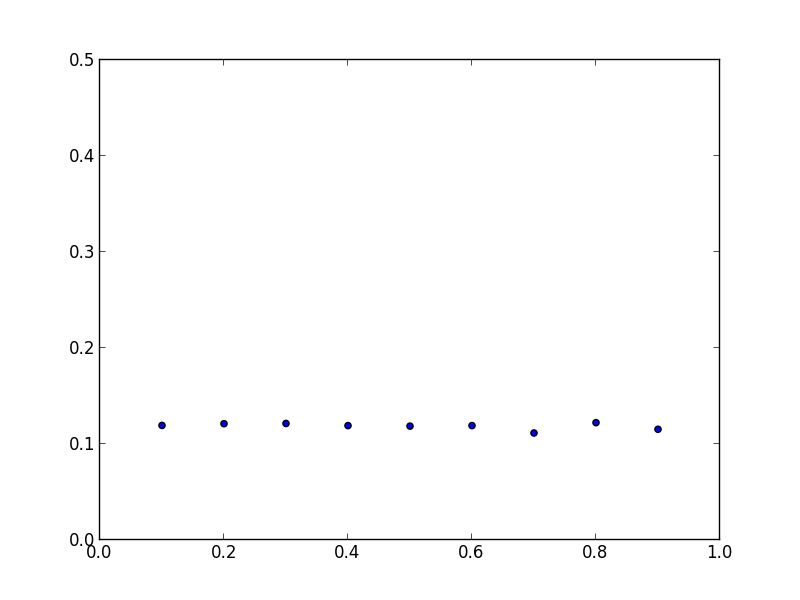
\includegraphics[width=\textwidth]{buyherd.png}
    \end{flushleft}
  \end{minipage}
  \begin{minipage}{0.5\textwidth}
    \begin{flushright}
      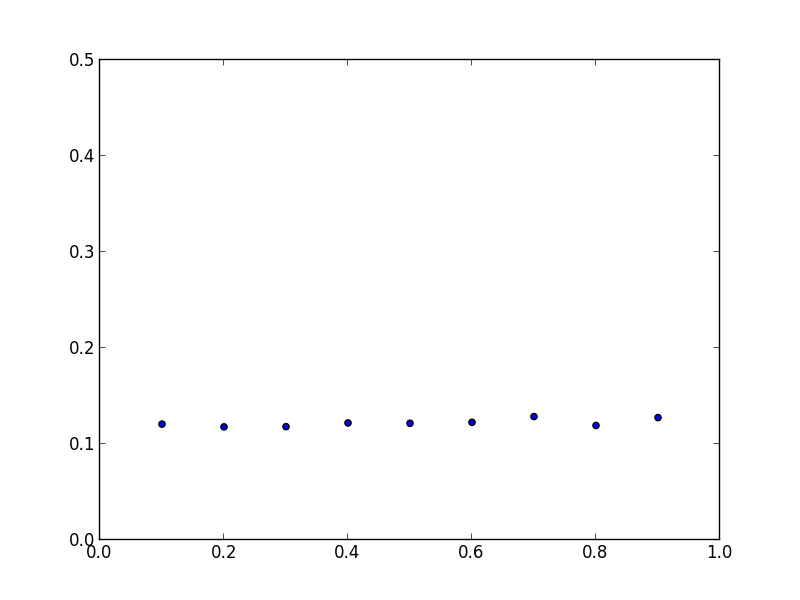
\includegraphics[width=\textwidth]{sellherd.png}
    \end{flushright}
  \end{minipage}
  \caption{Buy \& Sell herding using randomized signals}
\end{figure}

Figure 1 shows our results. 
Interestingly, we generated a uniform distribution of herding. 
The randomization was apparently enough to completely mitigate the effects of information risk on herding.
To some extent, this follows intuition: if private information is not predicatable, and varies in usefulness across time steps, then traders will be less likely to both ignore their own private information and to trust what is given to others.
That said, we did not run this simulation on nearly as many trials as Boortz et. al. did, nor did we use as many traders as they presumably used. 
However, it is still curious, and worth further investigation, that we find no evidence of the linear increase observed by the authors.

\subsection{Future Plans}
This simlation is only a first step.
We intend to run a more sophisticated model on real data.
Here we describe our plan for acquiring this data, a task which has proven suprisingly difficult.

We plan to acquire data either directly from the Chicago Mercantile Exchange (CME), or use the Interactive Brokers API for building our own dataset from market snapshot updates.
Interactive Brokers permits users to query for present data, but it does not offer historical datasets. 
Therefore we can build our own by plugging in to the API and gathering data over the course of the next month.

Our target market is the Forex market, specifically the top three most actively traded currency pairs: EUR/USD, USD/JPY, and GBP/USD.
We will look for market depth data, also known as L2 data, which will provide us the best bid/ask spreads, and also the 2nd, and 3rd price levels on both the buy and sell side.
Active traders have access to L2 market data, which means they have the ability to see when buyers or sellers are moving in some direction prior to the price movement by observing the change in the quantity at lower levels of the bid/ask book.
This public information is something traders can use when choosing whether to herd.

%% Talk about the graphs. The almgren graphs
Our analysis will plot the top bid and ask numbers, as well as a price-weighted average for the entire market available to us. 
We hope to find trends in the weighted average that influence the top prices. 
Trends in the weighted average should grow stronger in the presences of herding, driving the top numbers towards the trend.
We suspect that trading algorithms will take advantage of herd behavior to influence the price trend towards their goal, whether it be buying or selling.
In other words, we believe the algorithms will attempt to join and build a herd in order to maximize their objective.

\section{Discussion}
\subsection{Rationality of herding}
%% 2013-10-24: I am happy. Maybe cut this whole thing later but for now I am happy.
We have thus far considered herding the irrational, or at least unexpected behavior, assuming that investors follow their private information as the norm and degenerate into the herd mentality in exenuating circumstances.
Indeed, this is the the viewpoint contemporary models have embraced: herding is measured as deviation from some expected investment strategy, identified by similarity across different parties. 
One wonders whether this is a valid assumption. 
Making decisions based off the actions of fellow investors is not so far removed from making decisions based on publicly available information.
Historical trends, which are in effect what herd participants follow when making their decisions, are simply another form of public information. 
The herd mentality is more or less what we would expect to see in a completely fair market, without any information asymmetries. 
We might then refine the initial question to assume that herding will occur and instead ask how significant a role market trends play in investors' decision-making\textemdash if the herd action exerts a disproportionately large influence on buyer and seller behavior\textemdash but it seems strange, on review, to assume that players are not greatly influenced by their competitors actions.

%% In this spirit
Perhaps a better phemonena to explore are the circumstances in which an investor ignores \emph{public} information and instead follows private knowledge or intuition.
A contrary model, which instead of tracking similarity measures differences between investors, might provide more insight to the workings of these markets.  
Assuming that investors follow the public information and each others' decisions exclusively might permit us to draw conclusions about the influence or extent of participants' private information.
This is a naive investment strategy, subject to gaming and easily misled, but may in fact be a better generalization for how investors function in practice.

\subsection{Analyzing automatic traders}
%% about how we wish we could pin down the algorithm's criteria for choosing to her
Earlier, we expressed a desire to identify when trading algorithms choose to herd.
At first glance, this seems to be a feasible goal, and a possible topic for our full research paper. 
Indeed, we are interested in pursuing this topic, in analyzing algorithm performance on over time and making generalizations based on the conditions at the points when the various algorithms herded. 
If the automated traders are in fact following routines and not making randomized, noisy trades, then there must exist clear conditions where herding is beneficial, or at least conditions where an algorithm might perceive herding as the optimal strategy.
However, we cannot pursue this topic without a sufficient dataset.
We would need historical, high-frequency data (ticks every millisecond, at least) indicating price, quantity, and buyer in an active market. 

Unfortunately, data is what we are and have been lacking. 
Finding a single set of data, even anonymous data with ticks every second or less frequent, has been extremely difficult. 
Rather than continue to pursue what has been a disappointing and relatively fruitless endeavor, we will instead work to find a single dataset upon which we can test a herding model. 
Analysis of herding conditions for common (or rather, successful) algorithmic trading strategies must be delayed.

\section{Conclusion}
%% Summarize papers again
%% Summarize our thoughts, our contribution
%% Lay out future work
We have identified the topic of herding behavior in financial markets as a subject of interest, read a number of papers concerning this phenomena, and presented our reactions and open questions here.
In particular, we summarized Cont and Bouchad (2000), which provided a highly influential randomized model of commodities markets where herding occurs, and Boortz et. al., which sought to reconcile the theory and experimental results to date via a straightforward model tested on high-frequency data from the economic crisis.
Both works presented unique contributions to the field, taking a novel approach to the question. 
Yet herding is far from an explained phenomena.
The most pressing question, in our opinion, is to test a more intricate model on similar high-frequency data.
Hence a compelling avenue for our future research is to acquire high-frequency transaction data and run a new model on it.
We hope to explore this question in our main project.
%% that is a little ambitious

\bibliographystyle{amsplain}
\bibliography{reaction-paper}

\end{document}
